%%%%%%%%%%%%%%%%%%%%%%%%%%%%%%%%%%%%%%%%%%%%%%%%%%%%%%%%%%%%%%%%%%%%%%
% LaTeX Example: Project Report
%
% Source: http://www.howtotex.com
%
% Feel free to distribute this example, but please keep the referral
% to howtotex.com
% Date: March 2011 
% 
%%%%%%%%%%%%%%%%%%%%%%%%%%%%%%%%%%%%%%%%%%%%%%%%%%%%%%%%%%%%%%%%%%%%%%

\documentclass[paper=letter, fontsize=11pt]{article}
\usepackage[T1]{fontenc}
\usepackage{fourier}

\usepackage[english]{babel}															% English language/hyphenation
%\usepackage[protrusion=true,expansion=true]{microtype}	
\usepackage{amsmath,amsfonts,amsthm} % Math packages
\usepackage[pdftex]{graphicx}	
\usepackage{url}
\usepackage{siunitx}
\usepackage{subfig}
\usepackage{pgf}
\usepackage{float}



%%% Custom sectioning
\usepackage{sectsty}
\allsectionsfont{ \normalfont\scshape}


%%% Custom headers/footers (fancyhdr package)
\usepackage{fancyhdr}
\pagestyle{fancyplain}
\fancyhead{}											% No page header
\fancyfoot[L]{}											% Empty 
\fancyfoot[C]{}											% Empty
\fancyfoot[R]{\thepage}									% Pagenumbering
\renewcommand{\headrulewidth}{0pt}			% Remove header underlines
\renewcommand{\footrulewidth}{0pt}				% Remove footer underlines
\setlength{\headheight}{13.6pt}


%%% Equation and float numbering
\numberwithin{equation}{section}		% Equationnumbering: section.eq#
\numberwithin{figure}{section}			% Figurenumbering: section.fig#
\numberwithin{table}{section}				% Tablenumbering: section.tab#


%%% Maketitle metadata
\newcommand{\horrule}[1]{\rule{\linewidth}{#1}} 	% Horizontal rule

\title{
		%\vspace{-1in} 	
		\usefont{OT1}{bch}{b}{n}
		\normalfont \normalsize \textsc{State University at Buffalo} \\ [25pt]
		\horrule{0.5pt} \\[0.4cm]
		\Large Project 3 : Classification Algorithms \\
		\horrule{2pt} \\[0.5cm]
}
\author{
		\normalfont\large 								
        Yuze Liu \hspace{0.6cm}50207903\\
        \normalfont\large 
        Luting Chen \hspace{0.5cm}50133507\\
        \normalfont\large 
        Vicky Zheng \hspace{0.5cm}50037709\\
}
\date{\large 12/10/2016}
%%% Begin document
\begin{document}
\maketitle
%\newdimen\origiwspc%
\section{K-Nearest Neighbors Algorithm}
\subsection{Algorithm Description}
K-Nearest-Neighbors algorithm is a method used for classification and regression. In K-NN classification, the output will be the class membership. The objective will be classified by the majority votes of its neighbors, with the objective being assigned to the class most common among its k nearest neighbors.\\
In this project, we implement the 10-fold cross validation with the K-NN classify algorithm.\\
First,we split the whole dataset into 10 parts, we pick one part as the testing set and other 10 parts as the training set. For each sample in the testing set, we calculate the Euclidean distance between this sample to all the other samples in the training set. Then we pick the k nearest samples as its neighbors. We will classify this sample by the majority votes of that k neighbors.\\
In the project, there are only 2 classes. So we just need to compare the two weights.If the neighbor is classified as class 0, then the weight of this sample to be classified in class 0 will be : $weight0 = weight0 + \frac{1}{dis}$, dis is the Euclidean distance between the neighbors and the sample, other wise $weight1 = weight1 + \frac{1}{dis}$, then we compare weight0 and weight1 after go through all the neighbors of this sample, the sample will be classified with the higher weight.\\
After get the classification result from the test set, then we calculate all the four measurement values and then we pick another dataset from the remaining 9 datasets as the test set and other 9 as training set, repeat this procedure until all the ten datasets have been used as test set once.\\
In the end, we calculate the average of the four measurement values.  

\subsection{Pros and Cons}
Advantage:\\
The algorithm is effective when the dataset is very large.\\
The algorithm is robust to noisy training data.\\

\noindent Disadvantage:\\
Need to determine the value of parameter K.\\
There are a lot of choices to choose what kind of distance we will use to determine the neighbors.\\
Computation cost is quite high because we need to compute the distance of each query instance to all training samples.\\
If we have nominal data, we need to label the nominal value first and then calculate the distance.\\
\subsection{Result Evaluation}
\noindent \underline{Results for project3 dataset1.txt are}: \\ 
\textbf{Accuracy}: 0.92615914787\\
\textbf{Precision}: 0.922329566995\\
\textbf{Recall}: 0.87079481314\\
\textbf{F}: 0.89442003084\\

\noindent The above value is the optimal solution I get, k = 3\\

\noindent \underline{Results for project3 dataset2.txt are}:\\
\textbf{Accuracy}: 0.60625\\
\textbf{Precision}: 0.411791272453\\
\textbf{Recall}: 0.318770209838\\
\textbf{F}: 0.357137604338\\

\noindent The above value is the optimal solution I get, k = 4
\section{Decision Tree}
\subsection{Algorithm Description}
Decision Tree is a supervised learning method for classification. The goal is to create
a tree structured model that predicts the class of a test sample by learning decision
rules inferred from the data features. The decision rules are represented as internal
nodes in the tree. Each internal node denotes a test on an attribute, each branch denotes
the outcome of a test, and each leaf node holds a class label. When a new test
sample is needed to be classified, it goes down the decision tree from root to a leaf
node according to the rules stored in internal nodes and it's class label is determined
by the label stored in the leaf node. We implemented a 2-way-splitting decision tree
with prepruning.
\subsection{Implementation}
\paragraph{Preprocessing}In preprocessing, we made all attributes of different types to be
processable. For nominal attributes, we numbered them to make implementation easier. For example in dataset2, "Absent" was labeled as 0 and "Present" was labeled as 1. For continuous attributes, we discretized each of them into k bins and the
choice of k can be inferred by cross validation. A sample's feature is labeled 0 if
it's in the 1st bin, 1 if it's in the 2nd bin, 2 if it's in the 3rd bin and so on so forth,
until k-1 if it's in the kth bin. And it becomes an ordinal attribute because samples
labeled 0( landed in the 1st bin) are smaller than those labeled 1(landed in the 2nd
bin). So the order is: samples labeled 0 < samples labeled 1 < ... < samples labeled
k-1. Ordinal attributes can also be labeled as integers accordingly. As a result, after
preprocessing, all features will be represented as integers.

\begin{figure}[t]
  \centering
  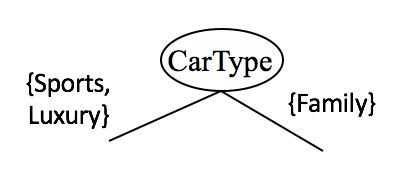
\includegraphics[width=0.8\linewidth,height=4cm]{f_fv.png}
  \caption{2 way splitting example}
\end{figure}

\paragraph{Splitting criterion} We used 2-way splitting to split tree nodes when it's needed
and we used misclassification error to compute the impurity of parent and children
nodes so as to choose the best splits. At tree node i, we tried out all possible 2-
way splits: we tried each attribute(f) and attribute value(fv) combination. And we
computed their corresponding impurity IMP: IMP = p * misclassificationError(leftChild) + (1-p) *misclassificationError(rightChild). p = $\frac{left{\_}node{\_}size}{parent{\_}node{\_}size}$. We got the minimum IMP and the corresponding feature f used to split as well as the
single feature value fv for one child node. In example Figure 2.1,  f is "CarType" and fv is "Family".

\paragraph{Terminating Criterion} The terminating criterions we used are listed below:
\begin{enumerate}
  \item current node has only one sample in the node.
  \item all points in the node have same label( impurity is 0).
  \item all points in the node's features are all the same.
  \item all possible splits's are bad: children's impurity > parent's impurity.
  \item the node's impurity is smaller than the threshold impurity (prepruning)
\end{enumerate}

When the threshold impurity is not 0, some nodes, whose impurity is smaller
than the threshold impurity, will stop splitting and become leaf nodes even though
they don't fulfill the first 4 criterions. Because the pruning doesn't happen after a full
tree is grown, this kind of pruning is called prepruning. When the threshold impurity
is 0, pruning is disabled.

If a node meets Criterion 4, it means no matter how we split the node, the resulting
impurity is always bigger than the original impurity. So, we think it is not
worthwhile to split this node. According to our experiments, a lot of leaf nodes with
only one sample will be created if we delete Criterion 4.

Except Criterion 1, all the other criterions may create leaf nodes whose class labels
are heterogeneous. We used majority vote to assign the label of heterogeneously
labeled leaf nodes.

\paragraph{Key function usage}  We designed three key functions to finish the pipeline of
decision tree classification. The input parameters are omitted for better readability
in the report.
\begin{enumerate}
  \item hunt(): learn the tree structure
  \item treenode{\_}list{\_}label(): majority vote each leaf node and get leaf node class labels
  \item assign{\_}labels(): classify new test samples according to the learned decision
tree
\end{enumerate}

\paragraph{Tree presentation}Our tree presentation is very humble. The tree grows from left to right: the root of
the leftmost node and each colunm is one level of the tree. For each internal node,
it follows the format of "[parent{\_}id] my{\_}id". For the root node, it's parent{\_}id is 0.
For each leaf node, it follows the format of "[parent{\_}id] my{\_}id:classLabel". Since for
Project 3, we only deal with 2 classes, leaf nodes are either "[parent{\_}id] my{\_}id:0" or
"[parent{\_}id] my{\_}id:1". We can also print out the samples each node includes as well
as internal nodes's splitting conditions. The following photo is an example. In the example Figure 2.2, node 1 is the root and it has 2 children node 2 and node 3;
node 1 is not a leaf node, so  it doesn't have the part ':0.0' or ':1.0';
node 2 is the leaf node and all data that goes to this node is labeled as 0;
node 3 is also a leaf node and all data that goes to this node is labeled as 1.

\begin{figure}[h]
  \centering
  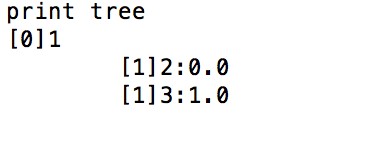
\includegraphics[width=0.8\linewidth,height=4cm]{tree_presentation_example.png}
  \caption{Tree Presentation Example}
\end{figure}

\subsection{Pros and Cons}
Advantage:\\
Decision tree is easy to interpret, because it can be seen as a set of decision rules. \\
At each internal node,  decision tree will choose the feature that yields the lowest children's impurity, so it has the ability of selecting the most discriminatory features.\\
Handling both continuous and discrete data.

\noindent Disadvantage:\\
Need to discrete data for some particular construction algorithm.\\
When dataset is small, it may yield large errors.\\
Without pruning, the full tree can be complicated and overfitting.
\subsection{Result Evaluation}
10 fold  cross validation average scores, bin size is 5.
\\
\noindent \underline{ Results for project3 dataset1.txt are}: \\ 
\textbf{Accuracy}: 0.87142857\\
\textbf{Precision}: 0.98375\\
\textbf{Recall}: 0.65409125\\
\textbf{F}: 0.77726096\\

\noindent \underline{ Results for project3 dataset2.txt are}: \\ 
\textbf{Accuracy}: 0.65217391\\
\textbf{Precision}: 0.39571429\\
\textbf{Recall}: 0.08718615\\
\textbf{F}: 0.13374561\\

The following is a small experiment on the effect of prepruning. For dataset2, if the threshold impurity is 0, we will have 49 nodes in the learned decision tree( the result  figure is big, so we exclude this figure). While when threshold is 0.3, there are  39 nodes and when threshold is 0.34, there are 23 nodes.
\begin{figure}[h]
  \centering
  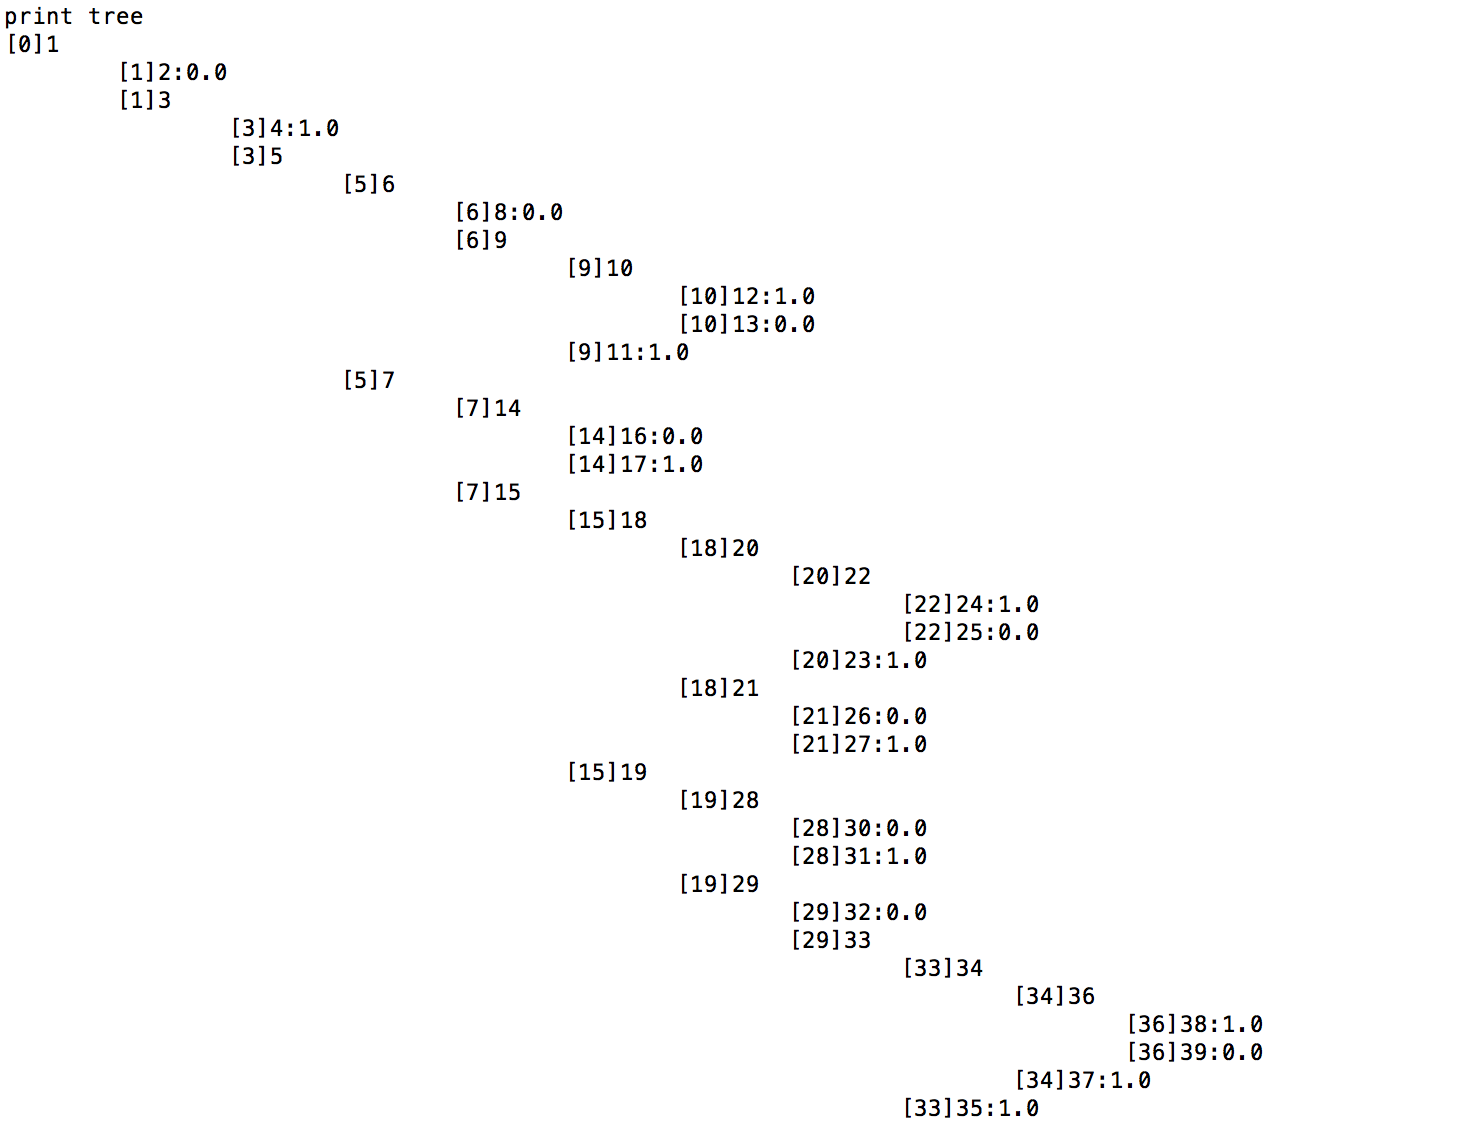
\includegraphics[width=1\linewidth,height=7cm]{dataset2_threshold_3.png}
  \caption{Prepuning with impurity threshold 0.3}
\end{figure}

\begin{figure}[h]
  \centering
  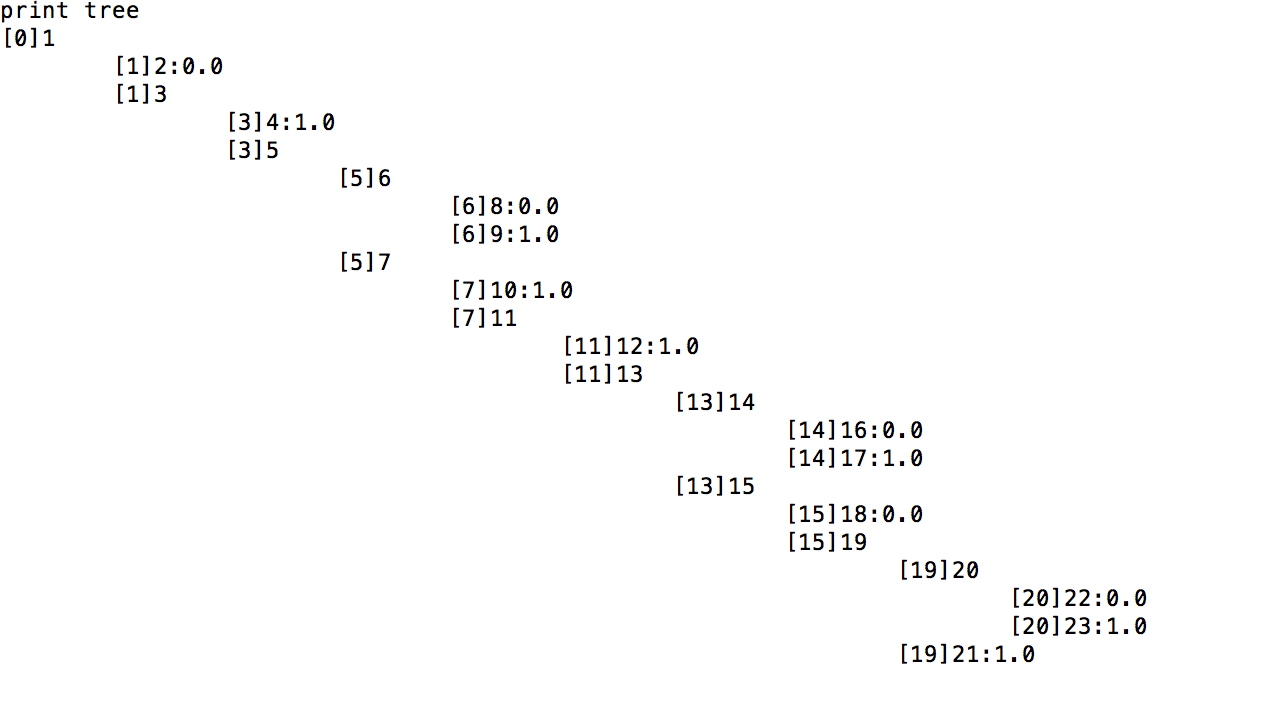
\includegraphics[width=0.8\linewidth,height=4cm]{dataset2_threshold_34.png}
  \caption{Prepuning with impurity threshold 0.34}
\end{figure}


\section{Decision Tree with Random Forest}
\subsection{Algorithm Description}
Decision tree with random forest is an ensemble learning method for classification.
Random forests can be built using bagging with random attribute selection at each
splitting node. For bagging, we randomly picked the same number of samples as the
training dataset with replacement and this is one round. We repeated the process for
n times and each round will generate a decision tree. We will get n decision trees in
the end and the class of a new test sample is determined by the equally weighted
voting among all learned decision trees.
\subsection{Pros and Cons}
Advantage:\\
tend to be more  accurate\\
no distribution assumptions\\
robust against outliers \\
 Because random forests consider many fewer attributes for each split, they are efficient
on very large databases\\
 \noindent Disadvantage:\\
 less efficient sampling compared to boosting\\
 
\subsection{Result Evaluation}
10 fold  cross validation average scores, bin size is 5, ensemble number is 5.
\\
\noindent \underline{ Results for project3 dataset1.txt are}: \\ 
\textbf{Accuracy}: 0.90535714\\
\textbf{Precision}: 0.9282444\\
\textbf{Recall}: 0.83087705\\
\textbf{F}: 0.86405575\\

\noindent \underline{ Results for project3 dataset2.txt are}: \\ 
\textbf{Accuracy}: 0.65652174\\
\textbf{Precision}: 0.51666667\\
\textbf{Recall}: 0.10631674\\
\textbf{F}: 0.16529107\\

\section{Decision Tree with Boosting}
\subsection{Algorithm Description}
Decision tree with random forest is also an ensemble learning method for classification.
The main differences between boosting and Random forest is boosting doesn't
have random feature selection when building trees and the final voting process for
new samples is weighted. The weights for each classifier is affected by its weighted
misclassification error. The following pseudocode Figure 4.1 describes how we implemented
boosting$\cite{textbook}$. Note when computing classifier weight $w_{i} = log\frac{1-error(M_{i})}{error(M_{i})}$, in case of "divided by zero" problem, we replaced a very small value like $1e^{-20}$ for 0 if  $error(M_{i})$= 0.
\begin{figure}[h]
  \centering
  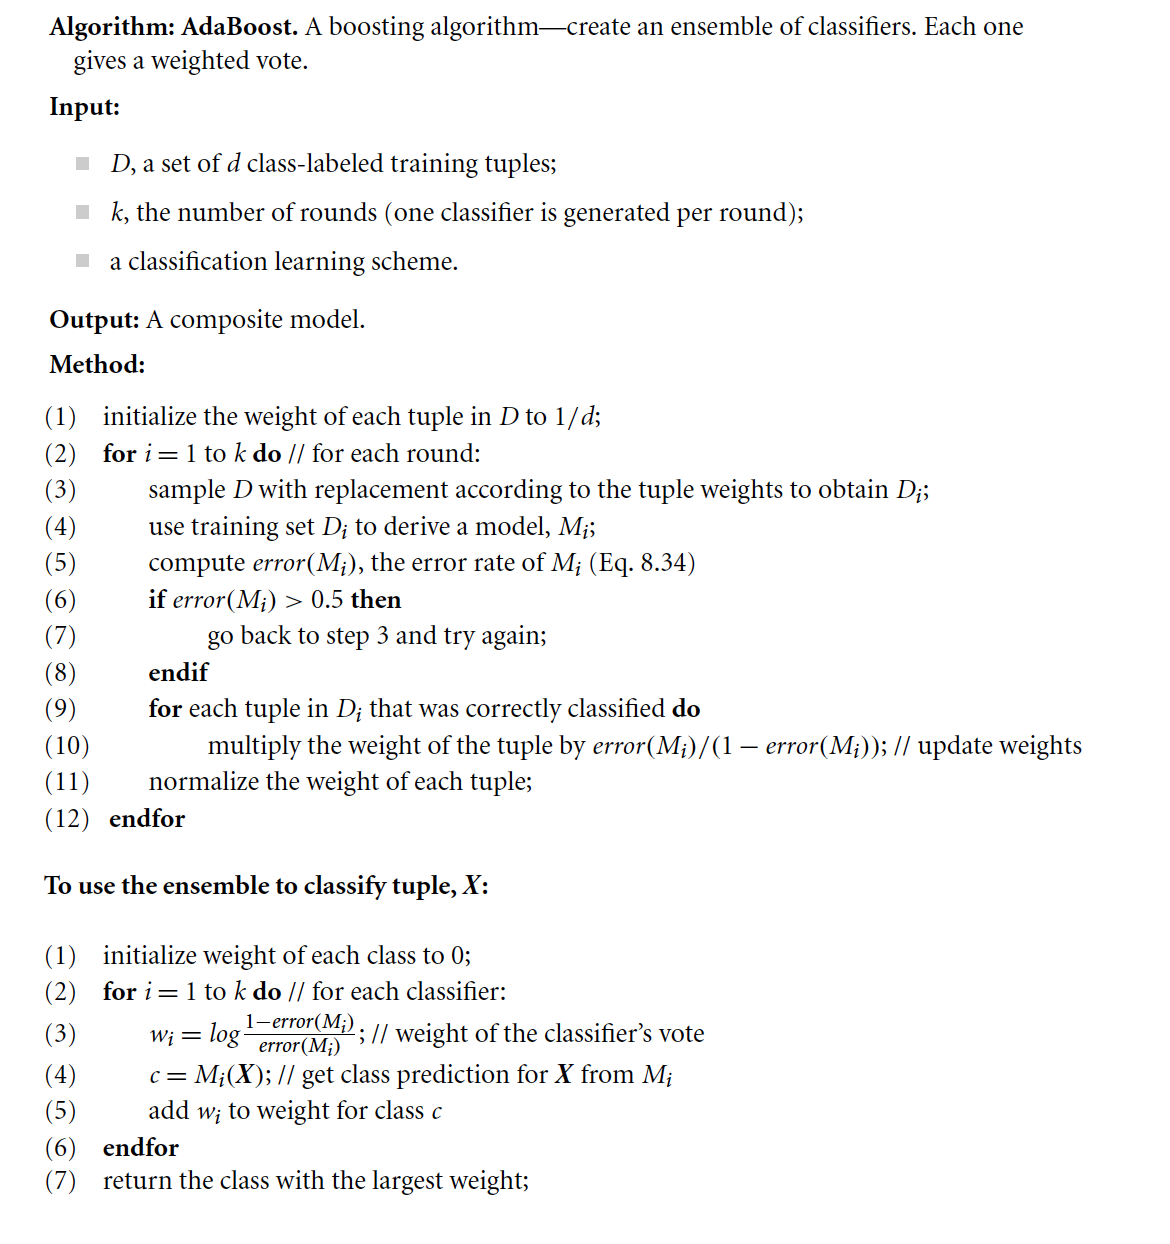
\includegraphics[width=0.8\linewidth,height=10cm]{boosting.png}
  \caption{Pseudocode for AdaBoosting}
\end{figure}


\subsection{Pros and Cons}
Advantage:\\
more accurate\\
very fast\\
\noindent Disadvantage:\\
tend to overfit
not as robust to errors and outliers
\subsection{Result Evaluation}
10 fold  cross validation average scores, bin size is 5, ensemble number is 5.
\\
\noindent \underline{ Results for project3 dataset1.txt are}: \\ 
\textbf{Accuracy}: 0.92678571\\
\textbf{Precision}: 0.92975827\\
\textbf{Recall}: 0.88075427\\
\textbf{F}: 0.89874908\\

\noindent \underline{ Results for project3 dataset2.txt are}: \\ 
\textbf{Accuracy}: 0.68913043\\
\textbf{Precision}: 0.61375791\\
\textbf{Recall}: 0.39169192\\
\textbf{F}: 0.44046561\\


\section{Naive Bayes}
\subsection{Algorithm Description}
Naive bayes is a classification algorithm that is based on the Bayes Theorem. Naive bayes aims to classify the probability of a sample $X$ being in a class $H_i$ using Bayes Theorem. The Bayes theorem is:\\
\begin{center} $P(H_i|X) = \frac{P(H_i)P(X|H_i)}{P(X)}$ \end{center}

\noindent The things that we are classifying often have multiple attributes which we will refer to as $A$ where $A = (A_1,A_2,...,A_d)$. Let $X$ be something we are trying to classify and $X = (x_1, x_2, ..., x_d)$. $P(X)$ is the prior probability of $X$ where $P(x_j) = \frac{n_j}{n}$ where $n_j$ is the number of of training samples in our training set that have the value $x_j$ for attribute $A_j$. 

% The probability that a given sample $X$ is in a class $H_i$ is: \begin{center} $P(H_i|X) = P(H_i|x_1)*P(H_i|x_2)*...*P(H_i|x_d)*P(H_i)$ \end{center}
$P(H_i)$ is simply the class prior probability. 

$P(X|H_i)$,the descriptor posterior probability, can be calculated by:

\begin{center} $P(X|H_i) = \prod_{i=1}^{d} P(x_j, H_i)$ \end{center}

\noindent Calculating the descriptor posterior probability reveals on of the weaknesses of Naive Bayes. If a single value $P(x_j, H_i)$ is 0 then the entire product of $P(X|H_i) = \prod_{i=1}^{d} P(x_j, H_i)$ will evaulate to 0 which will cause $P(H_i|X) = \frac{P(H_i)P(X|H_i)}{P(X)}$ to also evaluate to 0. This can be corrected by using a Laplacian correction where if there is an $n_j = 0$, then we will simply add 1 to every $n_j$ and increase the total number of samples to $n+k$ where $k$ is the number of possible values the attribute $A_j$ can take on. 

\noindent You will also notice that $P(H_i|X) = \frac{P(H_i)P(X|H_i)}{P(X)}$ does not work for continuous values because we cannot count continuous values to get posterior probabilities. I chose to address this by assuming a Gaussian distribution to use:

\begin{center} $P(H_i | x_j) = \frac{1}{\sqrt{2\pi\sigma_{H_i,x_j}^2}}e^{-\frac{1}{2}(\frac{H_i-\mu_{H_i,x_j}}{\sigma_{H_i,x_j}}^2)}$ \end{center}

\noindent I chose to use this method because it seemed to be one of the most popular methods out there for dealing with continuous values when implementing Naive Bayes. 

\noindent After we calculate $P(H_i|X) = \frac{P(H_i)P(X|H_i)}{P(X)}$ for all $H_i$, we assign X to the class $H_i$ where $P(H_i|X)$ is the maximum probability.

\subsection{Pros and Cons}
Some of the pros of using Naive bayes is that its simple to implement and it is efficent. One of the cons, however, is that it assumes attribute independence, which of course is not true for all datasets. Another con is that the descriptor posterior probability may evaluate to 0 - we have to prevent this by using a Laplacian correction. This can happen often in small datasets so Naive bayes performs best on large datasets. 

\noindent Something else that may be considered a con is that there are multiple ways to deal with continuous attributes. I chose to handle this by using Gaussian Naive Bayes. This may not perform well for other datasets that have different distributions. 

\subsection{Result Evaluation}
I implemented k-cross fold by randomly shuffling my dataset, and partitioning it into $k$ test sets and $k$ training sets. I took the average of the $k$ accuracy, precision, recall and F-values. \\

\noindent \underline{Results for project3 dataset1.txt are}: \\ 
\textbf{Accuracy}: 0.712582417582\\
\textbf{Precision}: 0.589052375343\\
\textbf{Recall}: 0.748140191881\\
\textbf{F}: 0.657284240816\\

\noindent \underline{Results for project3 dataset2.txt are}:\\
\textbf{Accuracy}: 0.671195652174\\
\textbf{Precision}: 0.51574025974\\
\textbf{Recall}: 0.761451858741\\
\textbf{F}: 0.612021438585\\


\section{Other clarification}
When calculating scores like recall, precision and F score, we may come across "divided by zero" problem. For example, to compute precision = $  \frac{truePositive}{truePositive + falsePositive}$, if the denominator is 0, it means both truePositive and falsePositive are 0, and truePositive is the numerator then we can just assign precision as 0. We solved "divided by zero" problem similarly for recall and F score.
 \begin{thebibliography}{1}
 \bibitem{textbook}
 Han, Jiawei, Jian Pei, and Micheline Kamber. Data mining: concepts and techniques. Elsevier, 2011.
 \end{thebibliography}


\end{document}